\documentclass[a4paper]{article}
\usepackage[english,spanish]{babel}
\usepackage[utf8]{inputenc}
\usepackage[T1]{fontenc}
\usepackage{verse}
\usepackage[noend]{algpseudocode}
\usepackage{listings}
%% Sets page size and margins
\usepackage[a4paper,top=3cm,bottom=3cm,left=3cm,right=3cm,marginparwidth=1.75cm]{geometry}
%% Useful packages
\usepackage{amssymb,amsmath,amsthm,amsfonts}
\usepackage{graphicx}
\usepackage[colorinlistoftodos]{todonotes}
\usepackage[colorlinks=true, allcolors=blue]{hyperref}

\newcommand{\verso}[1] {
\settowidth{\versewidth}{123456789012345678901234567890}%
\begin{minipage}[t]{\dimexpr\versewidth+1pt\relax}
\begin{verse}[\versewidth]
{\fontfamily{qzc}\selectfont\large
  #1
}
\end{verse}
\end{minipage}\bigskip
}

\title{Trabajo Práctico 2}
\author{Sebastián Cherny}



\begin{document}
\maketitle
\title{Sesgo y Error Cuadrático Medio - Ejercicio 1}
\\

Tomo como EMV de la muestra $\widehat{\theta}_n = max(X_1, X_2, ..., X_n)$ , dado que si el estimador es menor a eso la probabilidad de tener esos valores es $0$ y cuanto más grande sea a partir de ahí la probabilidad decae ya que el $\theta$ está dividiendo en la función de probabilidad (y es positivo).\\
Y el estimador basado en el primer momento será $\Tilde{\theta}_n = \dfrac{2}{n}*\sum\limits_{i=1}^n X_i$ que hace que su esperanza sea $\theta$ (por lo que es insesgado).\\
El estimador consideré como $\widehat{\theta}_n^{mod}$, modificando el EMV, es $\widehat{\theta}_n^{mod} = max(X_1, ..., X_n) + min(X_1, ..., X_n)$, que se puede ver que su esperanza es $\theta$ (la esperanza del primero es $\theta * n/n+1$ y la del otro con $\theta * 1/n+1$, resultando su suma $\theta$), siendo insesgado.\\

Hice funciones aparte para calcular los tres estimadores a partir de la muestra, por las dudas de estar tomando mal algún valor, que quede claro que cambiándolo ahí por la fórmula correcta se arregla todo (al principio me confundí y tomé el promedio del máximo y del mínimo, y luego para arreglar eso sólo lo cambié ahí y listo).

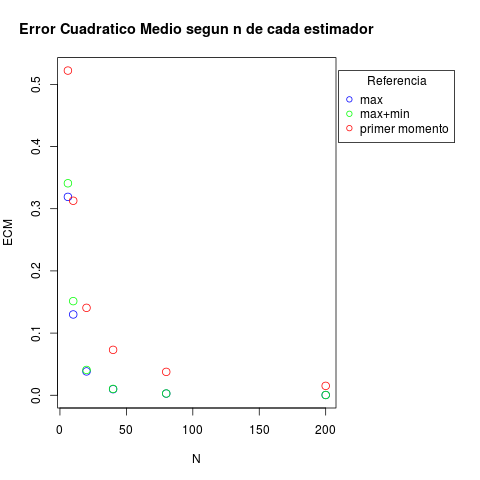
\includegraphics[width=12cm,height=9cm,keepaspectratio]{ejd.png}

No agregué los puntos de $n=500$ porque hacía que quedaran muy juntos los primeros valores de $n$. Se puede ver cómo el error cuadrático medio disminuye en todos los casos a medida que aumenta el $n$, en los tres casos con velocidad exponencial negativa, por lo que podríamos decir que a partir de un valor de $n$ ya no tiene sentido seguir aumentándolo ya que aumentará mucho el tiempo de ejecución y el ECM disminuirá muy poco. También se puede apreciar que el ECM tomando como estimador el que se basa en el primer momento es considerablemente mayor al ECM tomando los otros dos, que son parecidos.


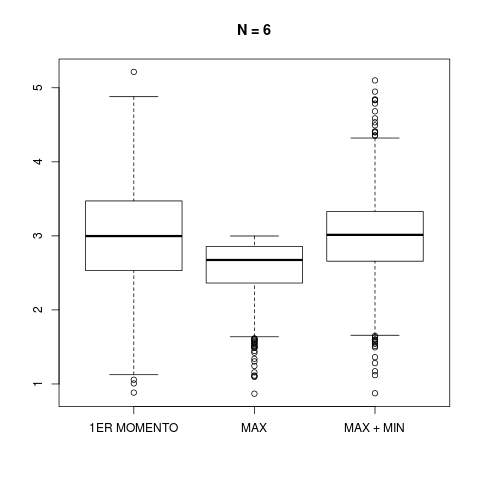
\includegraphics[width=5cm,height=9cm,keepaspectratio]{boxplot_6.png}
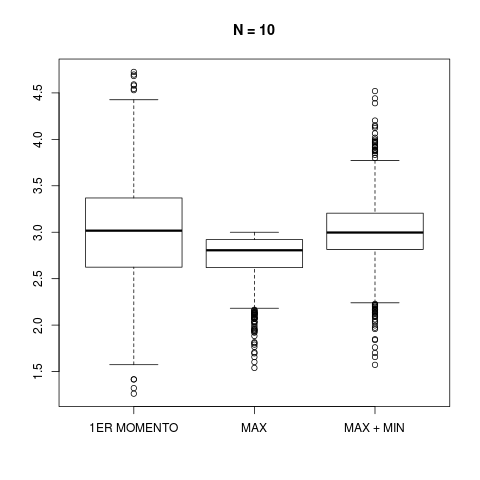
\includegraphics[width=5cm,height=9cm,keepaspectratio]{boxplot_10.png}
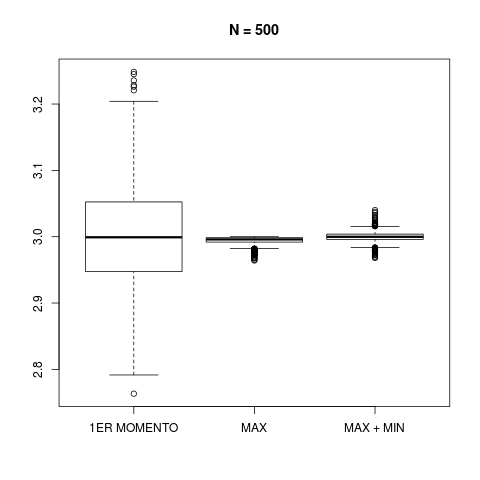
\includegraphics[width=5cm,height=9cm,keepaspectratio]{boxplot_500.png}

Acá se ven los boxplots para $N=6$, $N=10$, y $N=500$. Se puede ver para empezar que el esquema de los cuartiles y los 'outsiders' es similar en los tres casos para el estimador basado en el primer momento. Sin embargo, en los otros la caja se hace cada vez más chica, y en el EMV se ven todos los outsiders de un solo lado (que tiene sentido ya que se toma el máximo, no puede haber nada más arriba que $\theta_0 = 3$, y en el modificado (insesgado) se ve al igual que en el primero la simetría alrededor del promedio, que también en ambos casos coincide bastante bien que con $\theta_0$, mientras que el promedio del maximo va creciendo acercándose a $\theta_0$ \\

Tiene sentido esto que se ve de la simetría, ya que los estimadores primero y tercero en los gráficos ($\Tilde{\theta}_n$ y $\widehat{\theta}_n^{mod}$ respectivamente) son insesgados, pudiendo entenderse esto exactamente como la simetría alrededor de su promedio, ya que no tienen sesgo 'hacia ningún lado'. Mientras que el sesgo de $\widehat{\theta}_n$ es negativo, viéndose los valores de los estimadores un poco tirados 'hacia abajo'.


\end{document}